Electrochemical Impedance Spectroscopy (EIS) is a label-free, non-invasive technique for measuring the impedance value of an analyte in a large band of frequency \cite{Grossi2017,Sawhney2019}. EIS can be used in a plethora of applications, ranging from the monitoring of bacterial population growth \cite{Grossi2009}, to the analysis of body composition \cite{Jaffrin2008}, to the assessment of food quality \cite{Grossi2017}, metal corrosion \cite{McIntyre1996}, and battery charge \cite{diard1998eis}, to the specialized detection of cells, proteins and ions \cite{Xu2016}, to the investigation of bio-tissues non-invasively \cite{Zhang2018}. In its most basic form, EIS consists in injecting an AC sinusoidal waveform of a known voltage or current to a substance under test (SUT) and measuring its respective output current or voltage response, as shown in \autoref{fig:VoltageCurrent}. Since the amplitude and phase of the input signal is known, the impedance magnitude and phase components can then be deduced from the output response, as described in \autoref{eq:ImpedanceEIS}, \autoref{eq:Magnitude}, and \autoref{eq:Phase}. \par

Both a constant-valued voltage source and current source can be used as input for the impedance measurement, as illustrated in \autoref{fig:EIS_Galvano_potentio}. The former is termed “potentiostatic EIS” and the latter “galvanostatic EIS”. For most situation, these two techniques provide similar performance. There are, however, situations that favor one over the other, such as applications where the load voltage changes over time. Galvanostatic EIS would provide better results since the load voltage could then vary freely \cite{Grossi2017,Rajabzadeh2019EIS}. Galvanostatic EIS also benefits from an added convenience since the output is a voltage signal, which makes it easier to sample and manipulate compared to a current output.  \par
\begin{figure}[ht]
    \centering
    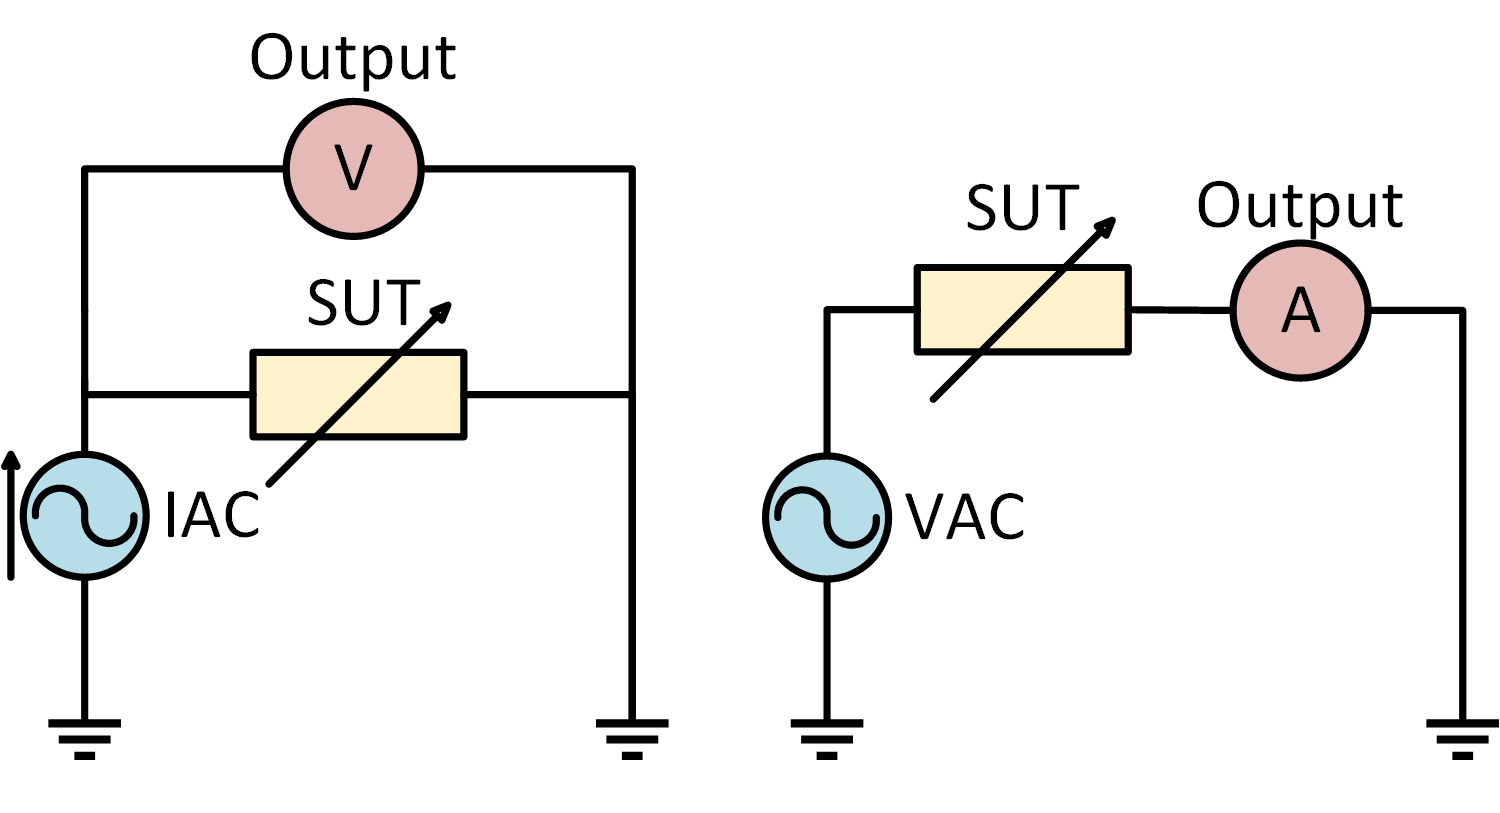
\includegraphics[width=0.8\textwidth]{EIS_Galvano_potentio}
    \caption{Galvanostatic (left) and potentiostatic (right) EIS.}
    \label{fig:EIS_Galvano_potentio}
\end{figure}

Sending sinusoidal waveforms of increasing frequency and repeatedly measuring the impedance using \autoref{eq:ImpedanceEIS} is an easy scheme for spectroscopy. This scheme results in a high Signal-to-Noise Ratio (SNR) \cite{leHuy2004circuits} but suffers from long measurement times which can be unacceptable for some applications \cite{Grossi2017,Kargupta2018,Rajabzadeh2019EIS}. This is the case since the impedance described in \ref{eq:ImpedanceEIS} is valid only for systems that have attained steady state. This means that a settling time is required before an impedance measurement can be deemed valid, to account for the transience of the system. The total transient time is a function of the system’s frequency response and the signal’s frequency. The settling time of the system itself should be low since the electronics used in its conception features fast response times (generally in the nanoseconds) \cite{horowitz1989art}. For low frequency applications, the settling time would depend mostly on the frequency of the input signal, which can be as low as a few millihertz for some applications \cite{Grossi2017}. \par

The precedent scheme can be called single-tone spectroscopy since the impedance is measured serially at fixed excitation frequencies. A higher throughput can be achieved using multi-tone spectroscopy \cite{horowitz1989art,Rajabzadeh2019Signals}. A broad-band excitation signals containing several frequency is coupled with discrete Fourier transform analysis to reduce the overall measurement time. However, additional care must be taken in order not to harm the SUT since the sum of multiple sinusoid results in a signal with a higher amplitude. In the end, the amplitude of the sinusoids at each frequency must be reduced and the phase must be chosen to minimize the Crest Factor (CF) \cite{landon1936study}. For that reason, the SNR of multi-tone spectroscopy is lower than that of single-tone spectroscopy. Rectangular pulses, Gaussian functions, sinc signals and chirp signals all are examples of such broad-band signals that can be used in multi-tone spectroscopy \cite{Grossi2017}. Pseudo random noise and Sigma-Delta Modulator ($\Sigma \Delta M$) \cite{reiss2008understanding} can also be used to produce the excitation signal; these two signals were tested by \citep{Rajabzadeh2019Signals}. The former tries to cover the entire frequency band of interest at once and the latter is a digitized variant of any analog signal such as the ones described previously. Pseudo random noise suffers from the same inconvenient as multi-tone and provides a satisfying spectrum only at the price of a high complexity; but since it is digitized, it is impervious to noise and can be multiplexed more easily. The same can be said of $\Sigma \Delta M$, it is however easier to implement and thus offers the better compromise between speed, precision, spectrum reliability and complexity \cite{Rajabzadeh2019Signals}. \par

Considering the broad range of applications permitted by impedimetric techniques, it is not surprising to find that the devices are heavily application specific. For example, the corrosion analysis of chemical coating is generally done at low frequency (a couple of hertz) \cite{Sawhney2019}, Impedance Microbiology (IM) is mostly done with a wide bandwidth that can begin as low as sub-hertz measurement and spans up to a couple hundred kilohertz, whilst whole-cell measurement is accomplished at Radio-Frequency (RF) ranging from Low Frequency (LF) to Very High Frequency (VHF) (30kHz to 300MHz) \cite{Xu2016,Opitz2019}. The impedances measured can be as low as a few milliohms and as high as tens of megaohms \cite{Grossi2017}. \par

Impedance, as described by \autoref{eq:ImpedanceEIS}, is defined for Linear Time Invariant (LTI) systems only. In order to be considered LTI, a system must respect the three conditions of linearity, stability and causality. Causality and Bounded-Input Bounded-Output (BIBO) stability are always respected for real-life systems in steady-states. However, linearity could pose a problem since most electrochemical systems are non-linear: the input signal should be of a low enough amplitude so as to operate in a pseudo-linear region (see \autoref{fig:smallEIS}) and no DC voltage or current should be added in order to minimize electrode-analyte polarization \cite{Grossi2017,Xu2016}. \par
\begin{figure}[ht]
    \centering
    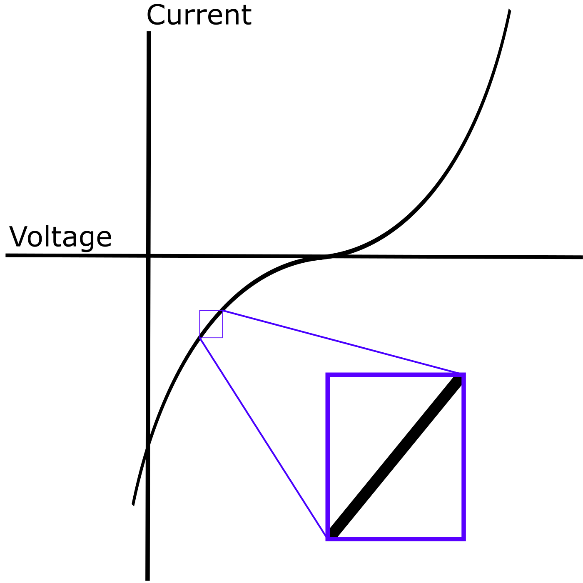
\includegraphics[width=0.5\textwidth]{smallEIS}
    \caption{Pseudo-linear region of electrochemical systems. Shows the principles of small perturbations for linear approximations.}
    \label{fig:smallEIS}
\end{figure}

To take into considerations these complicated needs, bench-top instruments such as LCR meters, Frequency Response Analyzer (FRA) and impedance analyzers offer performance extensive devices for impedimetric investigations in laboratory. These devices feature high accuracy, a broad band of available test frequency, configurations for two-, three- or four-electrodes modes (see \autoref{sec:ElectrodeDesign}) both for potentiostatic and galvanostatic EIS, and extensive software for complex modelling and data-fitting of the measured impedance. These devices are nevertheless \textbf{expensive, bulky, and energy-inefficient} which makes them unsuitable for portable measurements in the field \cite{Grossi2017,Chowdhury2017,Sawhney2019}. 